% !TeX program = xelatex
\documentclass[12pt]{article}
\usepackage[right=1.0in,left=1.0in,top=1.0in,bottom=1.0in]{geometry}
\usepackage{hyperref}
\hypersetup{colorlinks, citecolor=blue, filecolor=blue, linkcolor=blue, urlcolor=blue}
\usepackage{graphicx}
\usepackage{url}
\usepackage[round]{natbib}
\usepackage{amsmath,amsthm,amssymb}
\usepackage{booktabs}
\usepackage{multirow}
\usepackage{float}
\usepackage{pdflscape}
\usepackage[labelfont=bf,labelsep=period]{caption}
\usepackage{subcaption}
\usepackage{longtable}
\usepackage{threeparttable}
\usepackage{threeparttablex}
\usepackage{environ}

\usepackage{setspace}
\onehalfspacing

\let\textcite\citet

\graphicspath{{../results/figures/}}

% Appendix-style section/table/figure numbering (A.1, A.2, ...)
\renewcommand{\thesection}{\Alph{section}}
\renewcommand{\thetable}{\thesection.\arabic{table}}
\renewcommand{\thefigure}{\thesection.\arabic{figure}}
\renewcommand{\theequation}{\thesection.\arabic{equation}}

%%%%%%%%%%%%%%%%%%%%%%%%%%%%%%%%%%%%%%%%%%%%%%%%%%%%%%%%%%%%%

\title{Medical School Environments and Physician Treatment Styles \\[0.5em]
\large SUPPLEMENTAL APPENDIX}

\author{Shirley Cai\thanks{Emory University.} \and Ian McCarthy\thanks{Emory University.
\href{mailto:ian.mccarthy@emory.edu}{ian.mccarthy@emory.edu}}}

\date{\today}

%%%%%%%%%%%%%%%%%%%%%%%%%%%%%%%%%%%%%%%%%%%%%%%%%%%%%%%%%%%%%

\begin{document}

\maketitle

\section{Sample Construction Details}\label{sec:app-sample}

This section provides additional detail on the construction of our cardiologist-year analytical panel, the medical school-to-HRR crosswalk, the AHA training-period cath lab measure, and the NIH ExPORTER ranking panel.

\subsection{Cardiologist Assignment and Volume Restriction}

For each NSTEMI episode, we assign a single attending cardiologist following the procedure of \textcite{molitor2018}. The hierarchy prioritizes the first cardiologist who delivers a consultation (CPT codes 99251--99255 prior to their elimination by CMS in January 2010, with the hierarchy collapsing to first cardiologist of record for inpatient care for episodes thereafter), the first cardiologist of record on the inpatient stay, and the first cardiologist seen by the patient in carrier-line claims within 90 days of the index admission. We exclude episodes for which no cardiologist could be assigned and patient-years without Medicare fee-for-service coverage in every month of the admission year (or, for beneficiaries who die during the year, in every month through the month of death). Cardiologists are identified in MD-PPAS using primary-specialty fields for cardiology, interventional cardiology, clinical cardiac electrophysiology, and advanced heart failure and transplant cardiology.

We restrict to cardiologist-years with at least 11 NSTEMI patients. The threshold provides stable per-physician estimates of catheterization rates and aligns with the CMS cell-size threshold for public-use files. A trade-off of the volume restriction is that established, higher-volume cardiologists are over-represented in our analytical sample relative to the broader cardiologist population.

\subsection{Residualized Catheterization Rate}

Our outcome is the volume-weighted mean residualized cath-within-two-days indicator at the cardiologist-year level. At the patient level, we estimate a linear probability model regressing the cath-within-two-days indicator on age, sex, race, dual eligibility, the 31 Elixhauser comorbidity flags, and year fixed effects, retaining the residual as the patient-level outcome. We then aggregate to the cardiologist-year by taking the volume-weighted mean residual. The residualization removes mechanical variation across cardiologists that would arise from differences in patient comorbidity mix.

We construct the Elixhauser comorbidities by matching the diagnosis codes on the NSTEMI admission claim, by leading substring, to a lookup that maps ICD-9 and ICD-10 code prefixes to the 31 Elixhauser categories. A given diagnosis code may map to multiple Elixhauser categories, so the lookup is implemented as a join rather than a categorical recoding.

\subsection{Medical School-to-HRR Crosswalk}

The medical school HRR is constructed in three stages. First, we obtain each cardiologist's medical school name and graduation year from the CMS Physician Compare National Downloadable File. Second, we map medical school names to ZIP codes using a hand-curated crosswalk restricted to LCME-accredited U.S. allopathic medical schools, validated against the LCME accreditation directory. Of 187 medical schools in our crosswalk, 186 resolve via the LCME accreditation join, and one historically defunct school resolves via a separate fallback ZIP. Schools coded in Physician Compare as ``OTHER'' are excluded; the OTHER category captures most foreign-trained physicians and a small number of unmatched U.S. schools. Of the 11,942 cardiologists in the full Medicare panel, 5,847 (49\%, or 21,967 of 43,536 cardiologist-years) cannot be assigned a medical school HRR and are outside the analytical sample. Of these, 4,820 are coded OTHER in Physician Compare, 537 attended osteopathic schools, 389 attended schools that the crosswalk does not place, and 101 have no medical school recorded. Third, we map ZIP codes to hospital referral regions using the Dartmouth Atlas ZIP-to-HRR crosswalk (vintage 2015).

Our analytical panel restricts to allopathic MD graduates because only roughly 11\% of U.S. medical school graduates are osteopathic (DO), with an even smaller share among cardiologists (AAMC, U.S.\ Physician Workforce Data Dashboard).

\subsection{AHA Training-Period Cath Lab Measure}

Cath lab availability is recorded in the AHA Annual Survey CCLABHOS variable from 1994 onward and in the predecessor CCLAB82 variable from 1980--1993. Both are recoded to a binary indicator of direct hospital provision of cardiac catheterization. The HRR-year cath lab share is then computed as the share of AHA-respondent hospitals in each HRR-year for which the binary indicator equals one. The aggregated AHA series exhibits a smooth secular trend across the 1994 questionnaire revision, with the national HRR-mean cath lab share rising from approximately 0.14 in 1980 to approximately 0.39 in 2003. We interpret the smooth trend as evidence that the recoding from CCLAB82 to CCLABHOS does not introduce a measurement break.

For each cardiologist, we match the AHA HRR-year cath lab share at the year the cardiologist began medical school, defined as graduation year minus three, the year after matriculation. AHA cath lab data are available 1980--2003, so the year-matching produces clean assignments for cardiologists with graduation years 1983 through 2006. We restrict our analytical sample to this graduation-year window.

\subsection{Year-Matching and Cohort Variation}

Our preferred specification identifies $\beta_{\text{train}}$ off variation in cath lab availability across graduation cohorts who attended medical school in the same HRR. The variation comes from two sources. First, the rollout of cath labs occurred at different times across HRRs over the 1980--2003 period, so the same medical school HRR exposed different cohorts to different cath lab shares. Second, even within HRRs that had cath labs early, the share of hospitals offering cath services continued to rise across the rollout period. We rely on both sources of within-HRR temporal variation in our identification.

\subsection{NIH ExPORTER Ranking Panel}

To distinguish procedural exposure from medical school prestige, we build a year-matched panel of NIH research funding by medical school from the bulk files of the NIH ExPORTER database. We aggregate annual project-level award totals (1985--2025) to the medical school level using the institution-name field, with consolidation of name variants (abbreviations, mergers, renamings) by hand. Each medical school then receives a within-year rank in total NIH funding. The constructed series is validated against the published Blue Ridge Institute for Medical Research rankings, with a Pearson correlation across overlapping years above 0.99.

For each cardiologist, we match the medical school NIH rank in the year of medical school start (graduation year minus three), parallel to the AHA cath lab matching procedure. We use both continuous $-\log(\text{rank})$ and tier indicators (Top 10, Top 11--25, Top 26--50, Top 51--100, with unranked schools as the reference) in our specifications.

\subsection{GME Duration Filter}

We drop physician-years for which the implied training pipeline is incompatible with the cardiologist's observed graduation year and subspecialty. The required GME duration after medical school is six years for general cardiology, seven years for interventional cardiology, eight years for clinical cardiac electrophysiology, and seven years for advanced heart failure. Physician-years implying a training pipeline shorter than the GME duration are dropped. The filter removes approximately 70 of approximately 31,000 physician-year observations.

\section{Cross-Sectional Balance, by Subspecialty}\label{sec:app-balance}

Table~\ref{tab:app-balance-spec} reports the training-period cath lab share comparison between cross-sectional movers and stayers separately within each cardiology subspecialty, on the analytical sample of Table~2 in the main paper. The ordering matches Table~2 in every subspecialty, with movers coming from medical school HRRs with higher cath lab share than stayers in the same subspecialty, by 0.05 to 0.06 in general cardiology, interventional cardiology, and electrophysiology. The differences are statistically significant in general and interventional cardiology; electrophysiology and advanced heart failure have too few stayers (19 and 5 cardiologists) for a precise within-subspecialty test.

\begin{table}[htbp]
\centering
\begin{minipage}[h]{\textwidth}
  \caption{Cross-sectional balance by cardiology subspecialty}
  \label{tab:app-balance-spec}
  \centering
  \begin{tabular}{lcccccc}
  \toprule
   & \multicolumn{2}{c}{Stayers} & \multicolumn{2}{c}{Movers} & & \\
  \cmidrule(lr){2-3} \cmidrule(lr){4-5}
  Subspecialty & N & Train.\ cath & N & Train.\ cath & Diff. & $p$ \\
  \midrule
  General Cardiology     & 443   & 0.279 & 2,495 & 0.324 & 0.045 & $<$0.001 \\
  Interventional         & 117   & 0.274 & 715     & 0.333 & 0.060 & $<$0.001 \\
  Electrophysiology      & 33    & 0.291 & 185     & 0.357 & 0.065 & 0.046 \\
  Adv.\ Heart Failure    & 7     & 0.408 & 38      & 0.391 & $-$0.017 & 0.846 \\
  \bottomrule
  \end{tabular}
\end{minipage}
\end{table}

\section{Cohort-Trend Robustness}\label{sec:app-cohort}

The main text reports a linear graduation-year trend as the cohort-robustness check. Table~\ref{tab:app-cohort} reports the training imprint under the full set of cohort controls we consider, on the same within-origin sample. Columns (1) through (3) are the within-origin baseline and the baseline augmented with a linear and a quadratic graduation-year trend. Column (4) controls for the national cath lab share in the cardiologist's matriculation year, a measured national trend, so that the imprint is identified from how a region's cath lab availability deviates from the national rollout rather than from the rollout itself. The point estimate ranges between 0.053 and 0.066 across the four columns. Precision declines relative to the baseline because cath lab availability varies across both region and cohort, so any control for the cohort dimension absorbs part of the variation that identifies the imprint. We do not saturate the cohort dimension with graduation-year fixed effects, since doing so removes most of the within-HRR variation that identifies the training effect.

\begin{table}[htbp]
\centering
\begin{minipage}[h]{\textwidth}
  \caption[]{Training imprint under alternative cohort controls\footnote{The outcome is the volume-weighted mean residualized cath rate at the cardiologist-year level, on the within-origin sample. Column (1) is the within-origin baseline. Columns (2) and (3) add a linear and a quadratic graduation-year trend. Column (4) controls for the national cath lab share in the matriculation year. All specifications include medical school HRR, practice HRR, and year fixed effects, weight by NSTEMI volume, and cluster standard errors at the medical school HRR level. *** $p<0.01$, ** $p<0.05$, * $p<0.10$.}}
  \label{tab:app-cohort}
  \centering
  \begin{tabular}{lcccc}
\toprule
 & (1) & (2) & (3) & (4) \\
 & Baseline & Linear & Quadratic & Nat.\ share \\
\midrule
Training-HRR cath lab share & 0.058*** & 0.065** & 0.066** & 0.053* \\
 & (0.021) & (0.031) & (0.031) & (0.032) \\
\midrule
Graduation-year trend & None & Linear & Quadratic & None \\
National cath share & No & No & No & Yes \\
Med school HRR FE & Yes & Yes & Yes & Yes \\
Practice HRR FE & Yes & Yes & Yes & Yes \\
Year FE & Yes & Yes & Yes & Yes \\
Observations & 15,083 & 15,083 & 15,083 & 15,083 \\
\bottomrule
\end{tabular}


\end{minipage}
\end{table}

\subsection{Permutation Inference}

The within-origin estimate is identified from variation in training-period cath lab availability across graduation cohorts within a medical school HRR. We use two permutation tests to ask whether the actual pairing of cardiologists to training environments predicts later catheterization better than a random pairing. The first reshuffles cohorts within a region, and it has leverage only if training exposure genuinely varies within HRR across cohorts. It does. Of the total variance in training-period cath lab share across cardiologists, roughly 40\% is within medical school HRR across cohorts, a within-HRR standard deviation of 0.11 against a between-HRR standard deviation of 0.13, so reshuffling cohorts within a region moves the exposure measure over a wide range.

We reassign each cardiologist the training-period cath lab share that a different graduation cohort from the same medical school HRR actually faced, holding the outcome, the fixed effects, and the NSTEMI weights unchanged, and re-estimate the within-origin specification. Repeating this 1,000 times traces the distribution of the training coefficient under randomized cohort assignment. Panel (a) of Figure~\ref{fig:perm-null} plots the result. The permuted coefficient centers on zero, with 95\% of draws falling between $-0.039$ and 0.034. The actual estimate of 0.058 lies in the upper tail beyond all 1,000 permuted draws, for a two-sided randomization-inference $p$-value of 0.001. This is close to the clustered-SE $p$-value of 0.006 from the same specification, so the result does not rest on the cluster-robust asymptotics.

The second test holds each cardiologist's cohort fixed and reassigns the training-period cath lab share of a different medical school HRR in the same matriculation year, again holding the outcome, the fixed effects, and the NSTEMI weights unchanged. Panel (b) of Figure~\ref{fig:perm-null} plots the 1,000 permuted coefficients. Since the cath lab share rises across cohorts in every region, the permuted exposure retains the common cohort profile, and the permuted coefficients are centered on 0.015, with 95\% of draws falling between $-0.007$ and 0.036. The actual estimate of 0.058 exceeds all 1,000 draws, the largest of which is 0.054. The first test therefore indicates that the year of training matters within a region, and the second that the region of training matters within a year.

We read the permutation tests as evidence that the pairing of cardiologists to training environments is informative rather than an artifact of the limited within-region variation. They do not by themselves establish that the operative feature is cath lab availability as opposed to another regional attribute moving on the same cohort schedule, a distinction we take up through the subspecialty and rank results in the main text.

\begin{figure}[htbp]
\centering
\begin{minipage}[h]{\textwidth}
  \centering
  \caption[]{Permutation tests for the within-origin training imprint\footnote{Each histogram plots the training-period cath lab coefficient from 1,000 re-estimations of the within-origin specification. Panel (a) reassigns cardiologists the training-period cath lab share of a different graduation cohort from the same medical school HRR. Panel (b) reassigns cardiologists the share of a different medical school HRR in the same matriculation year. The dashed line marks zero and the solid line marks the actual estimate of 0.058. The outcome, fixed effects, and NSTEMI weights are held fixed across permutations.}}
  \begin{tabular}{cc}
  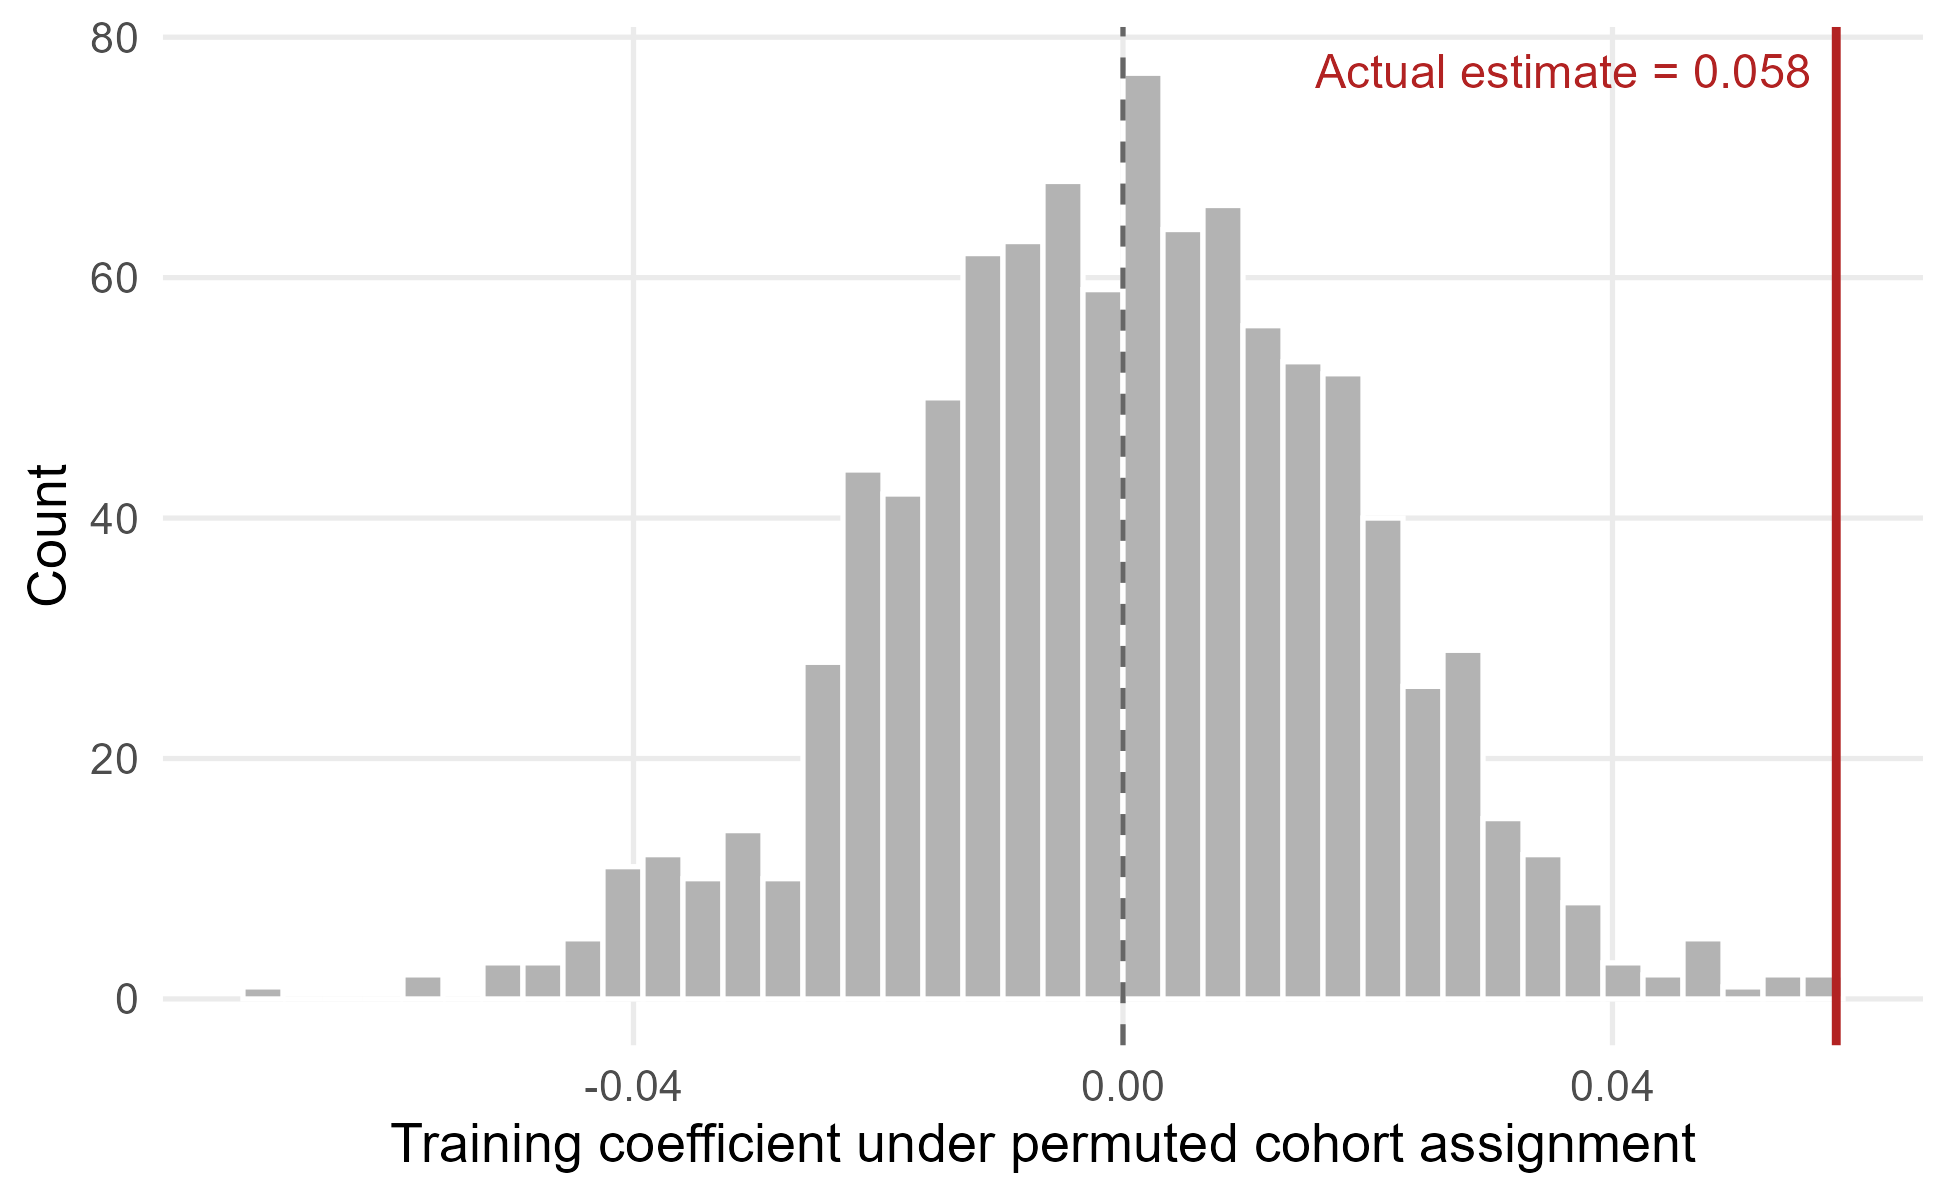
\includegraphics[height=4in,width=3.0in,keepaspectratio]{perm-null.png} &
  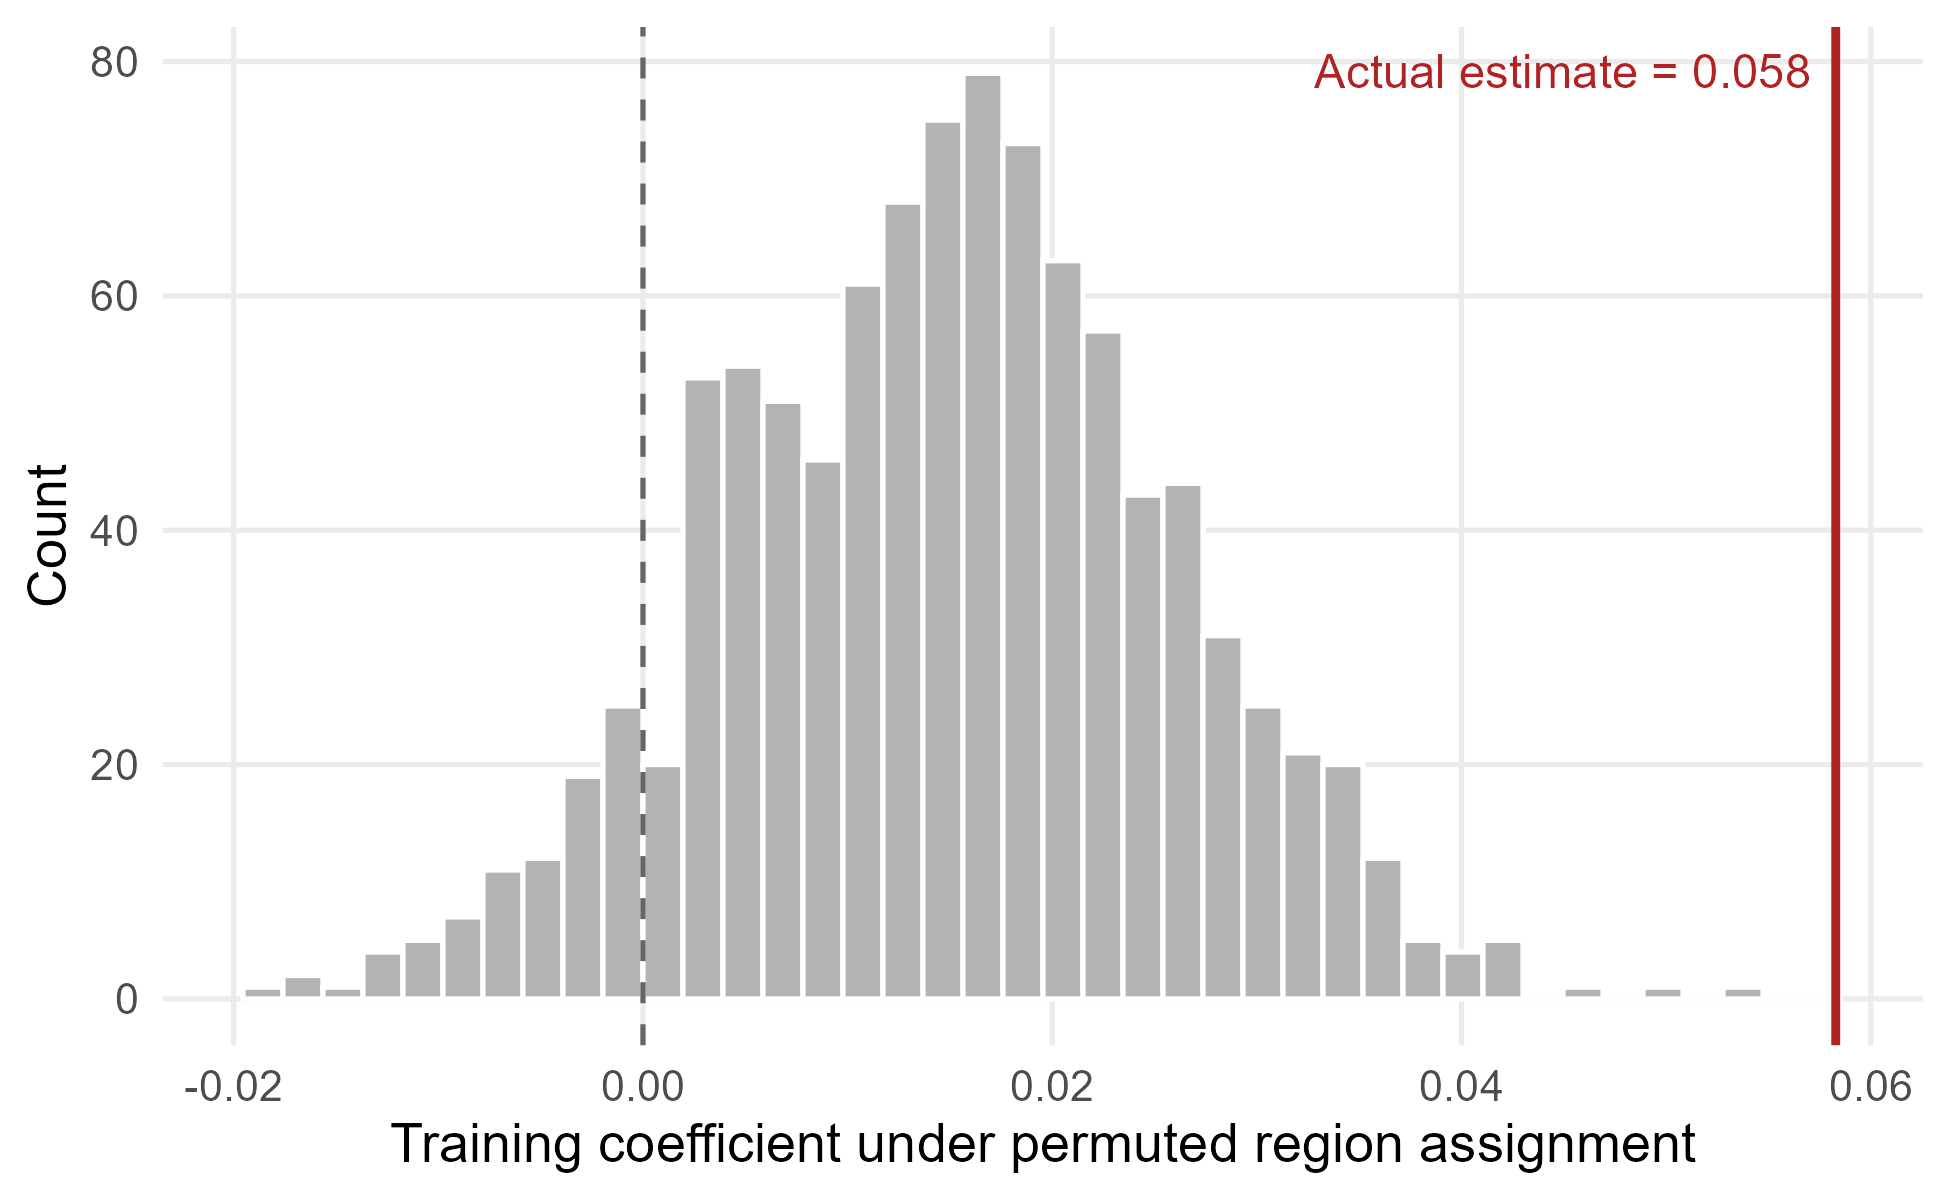
\includegraphics[height=4in,width=3.0in,keepaspectratio]{perm-null-region.png} \\
  (a) Cohorts reassigned within region & (b) Regions reassigned within cohort
  \end{tabular}
  \label{fig:perm-null}
\end{minipage}
\end{figure}

\section{Rank by Training-Period Cath Lab Share}\label{sec:app-rank}

The main paper documents that medical school NIH-funding rank does not predict later catheterization rates once training-period cath lab availability is included. Table~\ref{tab:app-rank-cells} splits cardiologists by Top-25 status and by whether their medical school HRR was above or below the median training-period cath lab share, with below-Top-25 schools in low-cath HRRs as the reference cell, and reports the cath rate in each of the other three cells relative to that reference.

\begin{table}[htbp]
\centering
\begin{minipage}[h]{\textwidth}
  \caption[]{Cath rate by medical school rank and training-period cath lab share\footnote{The outcome is the volume-weighted mean residualized cath rate at the cardiologist-year level. Cells cross Top-25 NIH rank status with whether the medical school HRR's training-period cath lab share is at or above the sample median. The specification includes practice HRR and year fixed effects, weights by NSTEMI volume, and clusters standard errors at the medical school HRR level. *** $p<0.01$, ** $p<0.05$, * $p<0.10$.}}
  \label{tab:app-rank-cells}
  \centering
  
\begin{tabular}{lcc}
\toprule
Cell (vs.\ Below Top 25 / Low cath) & $\hat{\beta}$ & (SE)\\
\midrule
Below Top 25 / High cath & 0.010** & (0.005)\\
Top 25 / Low cath & -0.000 & (0.006)\\
Top 25 / High cath & 0.017** & (0.007)\\
\midrule
Practice HRR FE & Yes & \\
Year FE & Yes & \\
Observations & 14,879 & \\
\bottomrule
\end{tabular}

\end{minipage}
\end{table}

\section{Doximity Match Procedure}\label{sec:app-doximity}

The main text uses Doximity profile data to test whether residency exposure adds to the medical school imprint. This appendix section documents the match procedure that links our Medicare cardiologists to Doximity profiles, maps Doximity training-program strings to AHA hospital identifiers, and constructs the residency-stage exposure measures used in that analysis.

\subsection{Doximity Profile Data}

Doximity (doximity.com) operates an online physician directory in which U.S. physicians can post professional profile pages. The profile pages report the physician's name, location, hospital affiliations, and credentials, along with structured fields for medical school, residency, and fellowship program names and graduation years. We work with the parsed profile fields that contain professional credentials, including the institution name and graduation year for each training stage, the cardiologist's current city and state, and gender. The profiles contain no patient-level information and no other identifiable personal data beyond the physician's professional credentials.

\subsection{Cardiologist Linkage}

The Doximity profiles do not include the National Provider Identifier, so we link cardiologists in our Medicare panel to Doximity profiles via normalized name, graduation year, and current practice state. We first normalize each side's name fields by transliterating to ASCII, lowercasing, stripping punctuation and credential suffixes (MD, DO, MPH, etc.), and collapsing whitespace. We then block on the normalized last and first name and apply a three-stage match.

Stage 1 retains pairs that are uniquely matched on normalized name from both sides. These represent the cleanest evidence of a real match. Stage 2 disambiguates pairs in which one cardiologist matches multiple Doximity profiles by name alone, using exact graduation-year agreement first, then state agreement, then exact medical-school string agreement. Stage 3 expands the candidate set for cardiologists not matched in Stage 1 or 2 using a small nickname canonicalization table (mapping common variants like Bob $\rightarrow$ Robert) and a first-initial fallback that requires exact graduation year and state agreement. Each downstream match must produce a one-to-one bipartite pairing.

Across all stages, the procedure matches 10,047 cardiologists from our Medicare panel, or roughly 80\% of cardiologists with non-missing name and graduation year in Physician Compare. The Stage-1 unique-name matches form the validation set for the linkage. Stage 1 used only first and last name and did not condition on graduation year, state, gender, or medical school. Across this validation set, we observe 99.2\% gender agreement, 86.5\% graduation-year agreement (with most disagreements within one year), 34.5\% practice-state agreement (consistent with Doximity profiles reflecting current practice in 2025--2026 while Physician Compare reflects practice locations in 2013--2018), and 29.1\% exact medical-school string agreement (with most disagreements reflecting formatting differences between sources rather than substantive disagreement). The strong gender and graduation-year agreement on orthogonal fields supports the validity of the name-based block.

\subsection{Doximity-to-AHA Hospital Mapping}

We map each Doximity training-program string to an AHA hospital identifier in three tiers. First, a hand-curated override table covers approximately 130 distinct training-program strings, including all programs that account for more than approximately 25 cardiologists in our matched sample. Each override pairs the Doximity program name with a canonical AHA name fragment and the state in which the program operates, and the override is resolved by searching the AHA roster within that state for the matching name fragment. Second, we attempt exact matches on the normalized hospital name between Doximity and AHA. Third, we apply a substring fuzzy match that requires the Doximity name to contain or be contained by an AHA hospital name, with a length-ratio guardrail of 3.0 to reject implausible alignments such as a short Doximity name matching a much longer AHA name. The cardiologist-level coverage of the three-tier procedure is roughly 48\% manual, 4\% exact, 18\% fuzzy, and 25\% unmatched on the residency side, with similar coverage on the fellowship side. We report the main residency-stage results both for the full matched sample and for the cleaner manual-plus-exact subsample, which drops the fuzzy-tier matches to test sensitivity to the noisier matches.

\subsection{Residency Exposure Measures}

For each matched cardiologist, we construct two residency-stage exposure measures from the AHA Annual Survey. The own-hospital cath measure is the mean of the AHA cath lab indicator at the cardiologist's residency hospital over their first three years of post-graduate training, where the years are derived from the cardiologist's medical-school graduation year and a three-year residency window. The same-HRR-system share measure is the mean across the same window of the share of cath-equipped hospitals among all hospitals in the same AHA-coded health system as the residency hospital, restricted to hospitals within the same hospital referral region. For residency hospitals not affiliated with a multi-hospital system, or whose system has only one hospital in the same HRR, the same-HRR-system share is set equal to the own-hospital cath measure.

\subsection{Direct-Exposure Test on Recent Graduates}\label{sec:app-recent-grad}

The AHA cath lab indicator is a coarse proxy for procedural exposure during residency. A sharper measure is the residency hospital's realized NSTEMI catheterization rate during the trainee's first three years of post-graduate training, constructed directly from the claims data. We implement this measure for cardiologists with medical-school graduation year 2006 or later, whose first three post-graduate years (PGY1--PGY3) overlap the 2008--2018 claims window. The recent-graduate subsample includes 351 cardiologists and 671 cardiologist-years, with a mean of 2.09 PGY years observed per cardiologist. After dropping singletons within fixed-effect cells, the within-origin column consists of 174 cardiologists. Table~\ref{tab:training-recent-grad} reports three specifications, progressing from practice-HRR and year fixed effects only (column~1) to the within-origin specification that adds medical-school HRR fixed effects (column~2) and a restriction to the cleaner manual-plus-exact residency-match subsample (column~3). The residency exposure coefficient is statistically indistinguishable from zero in all three columns. Point estimates are mildly negative but imprecisely estimated, and the confidence intervals do not support a positive residency imprint of the magnitude detected for medical school. The direct-exposure test on recent graduates corroborates the headline pipeline finding that the medical school imprint is not absorbed by residency exposure.

\begin{table}[htbp]
\centering
\begin{minipage}[h]{\textwidth}
  \caption[]{Residency cath rate and own catheterization, recent-graduate subsample\footnote{The outcome is the volume-weighted mean residualized cath rate at the cardiologist-year level. All columns include practice HRR and year fixed effects, with medical school HRR fixed effects added in columns (2) and (3), and weight by NSTEMI volume. Counts of cardiologist-years and cardiologists exclude singletons within fixed-effect cells. Standard errors are clustered at the cardiologist level in column (1) and at the medical school HRR level in columns (2) and (3). *** $p<0.01$, ** $p<0.05$, * $p<0.10$.}}
  \label{tab:training-recent-grad}
  \centering
  \begin{tabular}{lccc}
\toprule
 & (1) & (2) & (3) \\
 & Practice & Within & Manual+exact \\
 & HRR FE & origin & only \\
\midrule
Residency cath rate (PGY1-3) & \shortstack[c]{-0.058 \\ (0.064)} & \shortstack[c]{-0.145 \\ (0.118)} & \shortstack[c]{-0.184 \\ (0.168)} \\
\midrule
Cardiologist-years & 621 & 375 & 334 \\
Cardiologists & 307 & 174 & 153 \\
Practice HRR FE & Yes & Yes & Yes \\
Medical-school HRR FE & No & Yes & Yes \\
Year FE & Yes & Yes & Yes \\
\bottomrule
\end{tabular}


\end{minipage}
\end{table}

\section{Selection Diagnostics}\label{sec:app-ipw}

The main analysis addresses two distinct selection concerns. The first is that movers and stayers differ on observable characteristics, raising the possibility that the imprint estimate reflects mover-vs-stayer selection rather than a causal training effect. The second is that cardiologists from cath-rich training environments may systematically end up in cath-rich practice destinations, in which case our cross-sectional identification would conflate training imprint with destination-type sorting. We address the first with the inverse-probability-weighted (IPW) specification reported in the main paper. This section reports a parallel IPW exercise using a complementary measure of training-environment intensity, and a separate diagnostic for the destination-sorting concern. Section~\ref{sec:app-patient} reports balance of patient risk on training exposure, which addresses a third concern at the patient level.

\subsection{IPW Robustness Using the Peer-Cath Measure}

The main paper reports the IPW-weighted within-origin specification on the AHA training-period cath lab measure. Table~\ref{tab:app-selection-alt} reports a parallel IPW exercise using the leave-one-out peer cath rate in the medical school HRR as a complementary measure of training-environment intensity. The IPW weighting moves the imprint coefficient modestly relative to the unweighted baseline in column (1), in the same direction and of comparable magnitude to the shift we observe with the AHA measure in the main paper. Both exercises indicate that observable selection on graduation cohort, gender, subspecialty, and training-period intensity does not drive the imprint we estimate.

\begin{table}[htbp]
\centering
\begin{minipage}[h]{\textwidth}
  \caption[]{Selection robustness via inverse probability weighting (peer-cath measure)\footnote{The outcome is the volume-weighted mean residualized cath rate at the cardiologist-year level, estimated on the mover subsample. Both columns include practice HRR and year fixed effects and cluster standard errors at the medical school HRR level. Column (1) weights by NSTEMI volume; column (2) weights additionally by the inverse propensity of mover status. *** $p<0.01$, ** $p<0.05$, * $p<0.10$.}}
  \label{tab:app-selection-alt}
  \centering
  
\begin{tabular}{lcc}
\toprule
 & Baseline & IPW\\
\midrule
Med school HRR intensity & 0.093 & 0.095*\\
 & (0.058) & (0.057)\\
$\Delta$ intensity & 0.034 & 0.032\\
 & (0.031) & (0.030)\\
\addlinespace
Practice HRR FE & Yes & Yes\\
Year FE & Yes & Yes\\
IPW & No & Yes\\
\midrule\\
Observations & 18,527 & 18,527\\
\bottomrule
\end{tabular}

\end{minipage}
\end{table}

\subsection{Training Intensity and Destination Choice}\label{sec:app-train-dest}

A separate identification concern is that cardiologists from cath-rich training environments may end up in cath-rich current peer environments. If so, the training imprint we estimate in the main paper could partly reflect destination-type sorting on the training measure rather than a causal effect of training. To assess this directly, we regress each cardiologist's current peer cath rate (the leave-one-out residualized cath rate of other cardiologists in the same HRR-year) on their training-period cath lab share, with year fixed effects and clustering at the medical school HRR level.

On the full cardiologist-year panel (15,084 observations from 4,033 cardiologists with non-missing training-period and current-peer data), the coefficient on training-period cath lab share is $-$0.024 (SE 0.017), statistically indistinguishable from zero. Restricting to each cardiologist's earliest panel observation as a cross-section produces a similarly small estimate: $-$0.028 (SE 0.018), $n$ = 4,033. The pairwise correlation between training-period cath lab share and current peer cath rate is $-$0.05.

Training-period cath lab availability does not predict the current peer cath rate in our sample. Cardiologists from cath-rich training environments are not systematically located in cath-rich destinations, and the destination-type-sorting concern does not appear to drive our cross-sectional imprint estimate. We caution that our cardiologist-level cross-section uses the earliest panel observation rather than the first practice location after training, so this is a contemporaneous diagnostic rather than a direct test of training-induced sorting at first placement.

\section{Patient-Level Analysis}\label{sec:app-patient}

The main paper estimates the within-origin specification at the patient level to test whether the effect of training on catheterization differs by patient risk and whether the estimated increase in catheterization changes patient mortality. This section describes the sample and the risk measure underlying that analysis and reports the full set of patient-level estimates, including mortality by risk quintile.

\subsection{Sample and Risk Measure}

The patient-level sample is the set of NSTEMI inpatient stays assigned to the cardiologist-years in our analytical sample (246,053 stays treated by 4,033 cardiologists trained in 92 medical school HRRs). For each stay we observe the treating cardiologist's training-period cath lab share, medical school HRR, practice HRR, and leave-one-out practice-HRR cath rate in the year of admission. We measure baseline risk as the predicted one-year mortality from a logistic regression of death within 365 days of admission on age, age squared, sex, race, dual Medicare/Medicaid eligibility, months of dual eligibility, and the 31 Elixhauser comorbidity flags recorded on the index admission. We then split the predicted risk into quintiles, as summarized in Table~\ref{tab:app-patient-quintiles}. We see from the summary statistics that lower risk patients account for a larger share of catheterizations, and also the lowest subsequent mortality rates. Specifically, predicted one-year mortality rises from 0.095 in the lowest quintile to 0.555 in the highest, realized one-year mortality from 0.076 to 0.546, and the catheterization rate falls from 0.763 to 0.283.

\subsection{Imprint by Risk Quintile}

Table~\ref{tab:app-patient-risk} reports the effect of training exposure on catheterization, estimated at the patient level. Panel A reports the average effect from the specification in the main paper, and the coefficient of 0.058 (SE 0.020) in column (1) matches the cardiologist-level estimate. Column (2) adds admitting-hospital fixed effects, which absorb differences across hospitals in cath lab access and case mix within a practice HRR, and the coefficient falls to 0.039 (SE 0.016). Column (3) addresses a mechanical concern. Because the outcome is catheterization within two days, a patient who dies before then cannot be catheterized, so any effect of training on early death would appear as an effect on catheterization. Dropping patients who die within two days of admission leaves the coefficient at 0.060 (SE 0.020). Panel B interacts the training-period cath lab share with risk-quintile indicators and includes risk-quintile fixed effects in place of the individual patient covariates. The quintile coefficients range from 0.048 to 0.082 in the baseline specification and from 0.031 to 0.050 with hospital fixed effects. We also fail to reject a test of equality across quintile estimates ($p = 0.40$, $0.68$, and $0.51$).

\subsection{Mortality}\label{sec:app-patient-mortality}

Table~\ref{tab:app-patient-mortality} reports the effect of training exposure on 30-day mortality (column 1) and one-year mortality (column 2), averaged over all patients in Panel A and by risk quintile in Panel B. From Panel A, the coefficient on the training-period cath lab share is $-0.010$ for 30-day mortality (95\% CI $[-0.020, 0.001]$) and $-0.012$ for one-year mortality (95\% CI $[-0.032, 0.008]$). Both point estimates are therefore negative but small and imprecise, suggesting that training exposure has no meaningful effect on average, although we can rule out large mortality increases.

The estimates by quintile further show that the negative point estimates on average appear to be driven by effects among the lowest-risk patients. Specifically, in the two lowest quintiles, 30-day mortality falls by 0.011 (SE 0.005) and 0.023 (SE 0.008), while the estimates for the three higher quintiles are essentially centered around zero. That said, the five coefficients are also not distinguishable from one another ($p = 0.20$). The estimates on the lowest quintiles are small in absolute terms but larger relative to the baseline mortality of the patients in those quintiles, 2.0\% and 4.2\% (Table~\ref{tab:app-patient-quintiles}). At such baseline rates, a 10-percentage-point increase in exposure would lower 30-day mortality by about 5\% in each quintile. Still, we caution against interpreting these as causal mortality effects, since there is reason to suspect that the low-risk patients of higher-exposure cardiologists are healthier than their risk scores indicate.\footnote{In a placebo test, training exposure does not predict utilization in the year before admission on average, but among the lowest-risk patients, those treated by higher-exposure cardiologists had fewer inpatient stays and lower spending in the prior year. Adding those prior-year measures as controls leaves the mortality estimates unchanged, but the pattern suggests that these patients may differ in other ways as well.}

\begin{table}[htbp]
\centering
\begin{minipage}[h]{\textwidth}
  \caption[]{Analytical sample by quintile of predicted one-year mortality risk\footnote{NSTEMI episodes assigned to the cardiologist-years in the analytical sample, by quintile of predicted one-year mortality. Predicted risk is from a logit of death within 365 days on age, sex, race, dual eligibility, and the 31 Elixhauser comorbidities recorded on the index admission, fit on admissions through 2017 and scored for every episode, with quintiles cut over all NSTEMI episodes with an assigned cardiologist. Catheterization is within two days of admission. Thirty-day mortality is over admissions through December 1, 2018, and one-year mortality over admissions through 2017.}}
  \label{tab:app-patient-quintiles}
  \centering
  {\small \begin{tabular}{lccccc}
\toprule
 & & & & \multicolumn{2}{c}{Mortality} \\
\cmidrule(lr){5-6}
Risk quintile & Inpatient stays & \shortstack{Predicted \\ one-year \\ mortality} & \shortstack{Cath within \\ 2 days} & 30-day & One-year \\
\midrule
1 & 53,672 & 0.095 & 0.763 & 0.020 & 0.076 \\
2 & 51,625 & 0.154 & 0.708 & 0.042 & 0.133 \\
3 & 49,199 & 0.223 & 0.596 & 0.072 & 0.216 \\
4 & 46,857 & 0.323 & 0.441 & 0.125 & 0.339 \\
5 & 44,700 & 0.555 & 0.283 & 0.239 & 0.546 \\
\bottomrule
\end{tabular}

}
\end{minipage}
\end{table}

\begin{table}[htbp]
\centering
\begin{minipage}[h]{\textwidth}
  \caption[]{Patient-level training imprint, overall and by risk quintile\footnote{The outcome is an indicator for catheterization within two days of NSTEMI admission. Panel A reports the coefficient on the training-period cath lab share with patient controls (age, age squared, sex, race, dual eligibility, months of dual eligibility, and the 31 Elixhauser comorbidities). Panel B interacts the training-period share with risk-quintile indicators and replaces the patient controls with risk-quintile fixed effects. All columns include the leave-one-out practice-HRR cath rate and medical school HRR, practice HRR, and year fixed effects. Column (2) adds admitting-hospital fixed effects, and column (3) drops patients who die within two days of admission. The equality test is a Wald test that the five quintile coefficients are equal. Standard errors clustered at the medical school HRR. *** $p<0.01$, ** $p<0.05$, * $p<0.10$.}}
  \label{tab:app-patient-risk}
  \centering
  \begin{tabular}{lccc}
\toprule
 & (1) & (2) & (3) \\
\midrule
\multicolumn{4}{l}{\textit{Panel A. All patients}} \\
Training-HRR cath lab share & 0.058*** & 0.039** & 0.060*** \\
 & (0.020) & (0.016) & (0.020) \\
Observations & 246,053 & 245,405 & 241,748 \\
\midrule
\multicolumn{4}{l}{\textit{Panel B. By quintile of baseline mortality risk}} \\
Risk quintile 1 & 0.065*** & 0.050*** & 0.067*** \\
 & (0.022) & (0.017) & (0.022) \\
Risk quintile 2 & 0.048** & 0.031 & 0.050** \\
 & (0.023) & (0.019) & (0.023) \\
Risk quintile 3 & 0.055** & 0.035 & 0.059** \\
 & (0.026) & (0.021) & (0.026) \\
Risk quintile 4 & 0.068** & 0.040* & 0.070*** \\
 & (0.026) & (0.023) & (0.026) \\
Risk quintile 5 & 0.082*** & 0.048** & 0.082*** \\
 & (0.027) & (0.020) & (0.026) \\
Equal effects across quintiles ($p$-value) & 0.404 & 0.682 & 0.510 \\
Observations & 246,053 & 245,405 & 241,748 \\
\midrule
Medical-school HRR, practice HRR, year FE & Yes & Yes & Yes \\
Admitting hospital FE & No & Yes & No \\
Sample & All & All & Survived 2 days \\
Cardiologists & 4,033 & 4,033 & 4,033 \\
\bottomrule
\end{tabular}


\end{minipage}
\end{table}

\begin{table}[htbp]
\centering
\begin{minipage}[h]{\textwidth}
  \caption[]{Training exposure and patient mortality\footnote{Column (1) is death within 30 days of admission, for admissions through December 1, 2018, and column (2) is death within one year, for admissions through 2017. Panel A reports the coefficient on the training-period cath lab share with patient controls. Panel B interacts it with risk-quintile indicators and replaces the controls with risk-quintile fixed effects. All columns include the leave-one-out practice-HRR cath rate and medical school HRR, practice HRR, and year fixed effects. Standard errors clustered at the medical school HRR. *** $p<0.01$, ** $p<0.05$, * $p<0.10$.}}
  \label{tab:app-patient-mortality}
  \centering
  \begin{tabular}{lcc}
\toprule
 & 30-day mortality & One-year mortality \\
 & (1) & (2) \\
\midrule
\multicolumn{3}{l}{\textit{Panel A. Average effect}} \\
Training-HRR cath lab share & $-$0.010* & $-$0.012 \\
 & (0.005) & (0.010) \\
Observations & 244,836 & 229,106 \\
\midrule
\multicolumn{3}{l}{\textit{Panel B. By quintile of baseline mortality risk}} \\
Risk quintile 1 & $-$0.011** & $-$0.023** \\
 & (0.005) & (0.010) \\
Risk quintile 2 & $-$0.023*** & $-$0.018 \\
 & (0.008) & (0.015) \\
Risk quintile 3 & $-$0.004 & $-$0.002 \\
 & (0.008) & (0.014) \\
Risk quintile 4 & $-$0.012 & $-$0.013 \\
 & (0.011) & (0.014) \\
Risk quintile 5 & 0.003 & 0.003 \\
 & (0.013) & (0.018) \\
Equal effects across quintiles ($p$-value) & 0.198 & 0.506 \\
Observations & 244,836 & 229,106 \\
\midrule
Medical-school HRR, practice HRR, year FE & Yes & Yes \\
Cardiologists & 4,033 & 3,977 \\
\bottomrule
\end{tabular}


\end{minipage}
\end{table}

\clearpage

\section{Event-Study Details}\label{sec:app-es}

This section reports the full coefficient table for the within-physician event study around mid-career moves.

Table~\ref{tab:app-es-coefs} reports point estimates, standard errors, and 95\% confidence intervals for each event-time coefficient $\hat\beta_\tau$ in the within-physician event study, with $\tau \in [-3, 5]$ and $\tau = -1$ omitted as the reference period. The pre-move coefficients ($\tau \in \{-3, -2\}$) are statistically indistinguishable from zero, consistent with the parallel-trends assumption. Adaptation jumps at $\tau = 0$ to 0.496 (SE 0.078, 95\% CI [0.34, 0.65]). The post-move coefficients decline gradually from 0.325 at $\tau = 1$ to 0.214 at $\tau = 5$, and the $\tau = 5$ coefficient is not statistically distinguishable from zero ($p = 0.10$), but the confidence intervals from $\tau = 1$ onward all contain the pooled post-move coefficient, so the path is consistent with a flat post-move level.

\begin{table}[htbp]
\centering
\begin{minipage}[h]{0.85\textwidth}
  \caption[]{Event-study coefficients, within-physician adaptation around mid-career moves\footnote{Coefficients from the within-physician event study around mid-career moves described in the main text. The specification includes cardiologist and calendar-year fixed effects, weights by NSTEMI volume, and clusters standard errors at the cardiologist level. Event time $\tau$ is measured in years relative to the move year, with $\tau=-1$ the omitted reference period.}}
  \label{tab:app-es-coefs}
  \centering
  \begin{tabular}{lccccc}
  \toprule
  Event time $\tau$ & Estimate & SE & 95\% CI lo & 95\% CI hi & $p$-value \\
  \midrule
  $-3$ & $-$0.100 & 0.107 & $-$0.31 & 0.11 & 0.352 \\
  $-2$ & 0.034  & 0.091 & $-$0.14 & 0.21 & 0.704 \\
  $-1$ & 0       &       &         &      & ref.  \\
  $0$  & 0.496  & 0.078 & 0.34    & 0.65 & $<$0.001 \\
  $1$  & 0.325  & 0.086 & 0.16    & 0.49 & $<$0.001 \\
  $2$  & 0.325  & 0.103 & 0.12    & 0.53 & 0.002 \\
  $3$  & 0.305  & 0.104 & 0.10    & 0.51 & 0.004 \\
  $4$  & 0.288  & 0.113 & 0.07    & 0.51 & 0.011 \\
  $5$  & 0.214  & 0.131 & $-$0.04 & 0.47 & 0.102 \\
  \bottomrule
  \end{tabular}
\end{minipage}
\end{table}

Pre-trends are formally tested by the joint $F$-statistic on $\hat\beta_{-3}$ and $\hat\beta_{-2}$, which fails to reject the null of zero pre-trends at conventional levels. The post-move pooled coefficient (constraining $\beta_\tau = \beta$ for $\tau \geq 0$) is 0.403, which we use in the cohort-transition calibration in the main paper.

\section{Cohort-Transition Simulation}\label{sec:app-var}

The main paper combines $\hat\beta_{\text{train}} = 0.058$ and $\hat\beta_{\text{dest}} = 0.403$ into a steady-state multiplier of approximately 1.67. This section reports the derivation of the multiplier and the cohort-transition path implied by gradual cohort replacement.

\subsection{Derivation of the Long-Run Multiplier}

The multiplier in the main paper rests on three assumptions. First, the destination response operates linearly on the peer mean, so that a one-percentage-point shift in peer-environment cath rate raises own cath rate by $\beta_{\text{dest}}$ percentage points. Second, the system reaches a steady state in which the peer mean equals the average own cath rate across all cardiologists in the HRR. Third, all cohorts contribute equally to the peer mean once the transition is complete. Let $\bar{y}$ denote the steady-state per-cardiologist cath rate and $\Delta\tau$ the uniform training-period cath lab shift. Each cardiologist's steady-state cath rate equals their direct training imprint plus their adaptation to the peer mean,
\begin{equation*}
\bar{y} = \beta_{\text{train}} \cdot \Delta\tau + \beta_{\text{dest}} \cdot \bar{y},
\end{equation*}
which solves to
\begin{equation*}
\bar{y} = \frac{\beta_{\text{train}} \cdot \Delta\tau}{1 - \beta_{\text{dest}}}.
\end{equation*}
The multiplier $1/(1 - \beta_{\text{dest}})$ captures the cumulative peer-effect spillover that accumulates as new cohorts displace old ones and incumbents adjust to the evolving peer environment.

\subsection{Cohort Transition Path}

We trace the per-cardiologist response to a uniform 10-percentage-point increase in training-period cath lab share for all newly entering cohorts, holding the cohort-replacement rate at 5\% per year (corresponding to a 20-year career length). Each year, the share of cohorts that received the training shift rises by 5 percentage points until the entire cohort distribution has been replaced at year 20. The cardiologist-level cath rate evolves according to
\begin{equation*}
y_t = \beta_{\text{train}} \cdot \Delta\tau \cdot \text{share}_t + \beta_{\text{dest}} \cdot y_{t-1},
\end{equation*}
with the direct training effect compounding through the destination feedback loop. The path approaches the long-run multiplier $1/(1 - \beta_{\text{dest}}) = 1.67$ asymptotically under our within-physician estimate of $\beta_{\text{dest}} = 0.40$. Roughly half of the long-run effect is realized within ten years of the shock, and the system reaches about 97\% of steady state by year 20.

\clearpage

%%%%%%%%%%%%%%%%%%%%%%%%%%%%%%%%%%%%%%%%%%%%%%%%
\begin{singlespace}
\bibliographystyle{aer}
\bibliography{BibTeX_Library}
\end{singlespace}
%%%%%%%%%%%%%%%%%%%%%%%%%%%%%%%%%%%%%%%%%%%%%%%%

\end{document}
